\documentclass[12pt]{article}


\usepackage{amssymb}
\usepackage{amsmath}
\usepackage{fullpage}
\usepackage{epsfig}
\usepackage{epstopdf}
\everymath{\displaystyle}
\usepackage{enumerate}

\newif\ifans

\ansfalse

\begin{document}

\begin{center}
\underline{\LARGE{Double Integrals Over Rectangular Regions}}
\end{center}

\noindent SUGGESTED REFERENCE MATERIAL:

\bigskip

\noindent As you work through the problems listed below, you should reference Chapter 14.1 of the recommended textbook (or the equivalent chapter in your alternative textbook/online resource) and your lecture notes.

\bigskip

\noindent EXPECTED SKILLS:

\begin{itemize}

\item Be able to compute double integral calculations over rectangular regions using partial integration. 

\item Know how to inspect an integral to decide if the order of integration is easier one way ($y$ first, $x$ second) or the other ($x$ first, $y$ second). 

\item Kow how to use a double integral as the volume under a surface or find the area or a region in the $xy$-plane.

\end{itemize}

\noindent PRACTICE PROBLEMS:

\medskip

\noindent {\bf For problems 1-4, evaluate the given iterated integral.}

\begin{enumerate}

\item $\int_0^1\int_0^2\left(3x^3-y^2+2\right)\,dx\,dy$

\ifans{\fbox{$\frac{46}{3}$}} \fi

\item $\int_0^2\int_1^3 x^2y\,dy\,dx$

\ifans{\fbox{$\frac{32}{3}$}} \fi

\item $\int_0^{\ln{4}}\int_0^{\ln{5}}e^{x+y}\,dy\,dx$

\ifans{\fbox{$12$}} \fi

\item $\int_0^{\pi} \int_1^2 x\sin{y} \,dx \,dy$

\ifans{\fbox{$3$}} \fi

\item Consider $f(x,y)=x^2+y^2$ and $R:[0,4]\times[0,4]$.

\begin{enumerate}

\item Estimate the volume bounded between the graph of $f(x,y)$ and the $xy$-plane over the region $R$ using 4 subrectagles of equal area and choosing the lower left hand corners as the sample points.

\ifans{\fbox{$64$}} \fi

\item Estimate the volume bounded between the graph of $f(x,y)$ and the $xy$-plane over the region $R$ using 4 subrectagles of equal area and choosing the upper right hand corners as the sample points.

\ifans{\fbox{$320$}} \fi

\item Estimate the volume bounded between the graph of $f(x,y)$ and the $xy$-plane over the region $R$ using 4 subrectagles of equal area and choosing the middle of the rectangle as the sample points.

\ifans{\fbox{$160$}} \fi

\item Compute the exact volume of the solid bounded between $f(x,y)$ and the $xy$-plane over the region $R$ using an appropriate double integral.

\ifans{\fbox{$\frac{512}{3}$}} \fi

\end{enumerate}

\item Each of the following iterated integrals represents the volume of a solid.  Make a sketch of a solid whose volume is represented by the integral.  

\begin{enumerate}

\item $\int_0^4 \int_1^3 {5} \,dy \,dx$

\ifans{\fbox{\parbox{1\linewidth}{This value of this integral can be thought of as the volume between the $z=5$ plane and the $xy$-plane over the rectangle $[0,4]\times[1,3]$.\\
\begin{center}
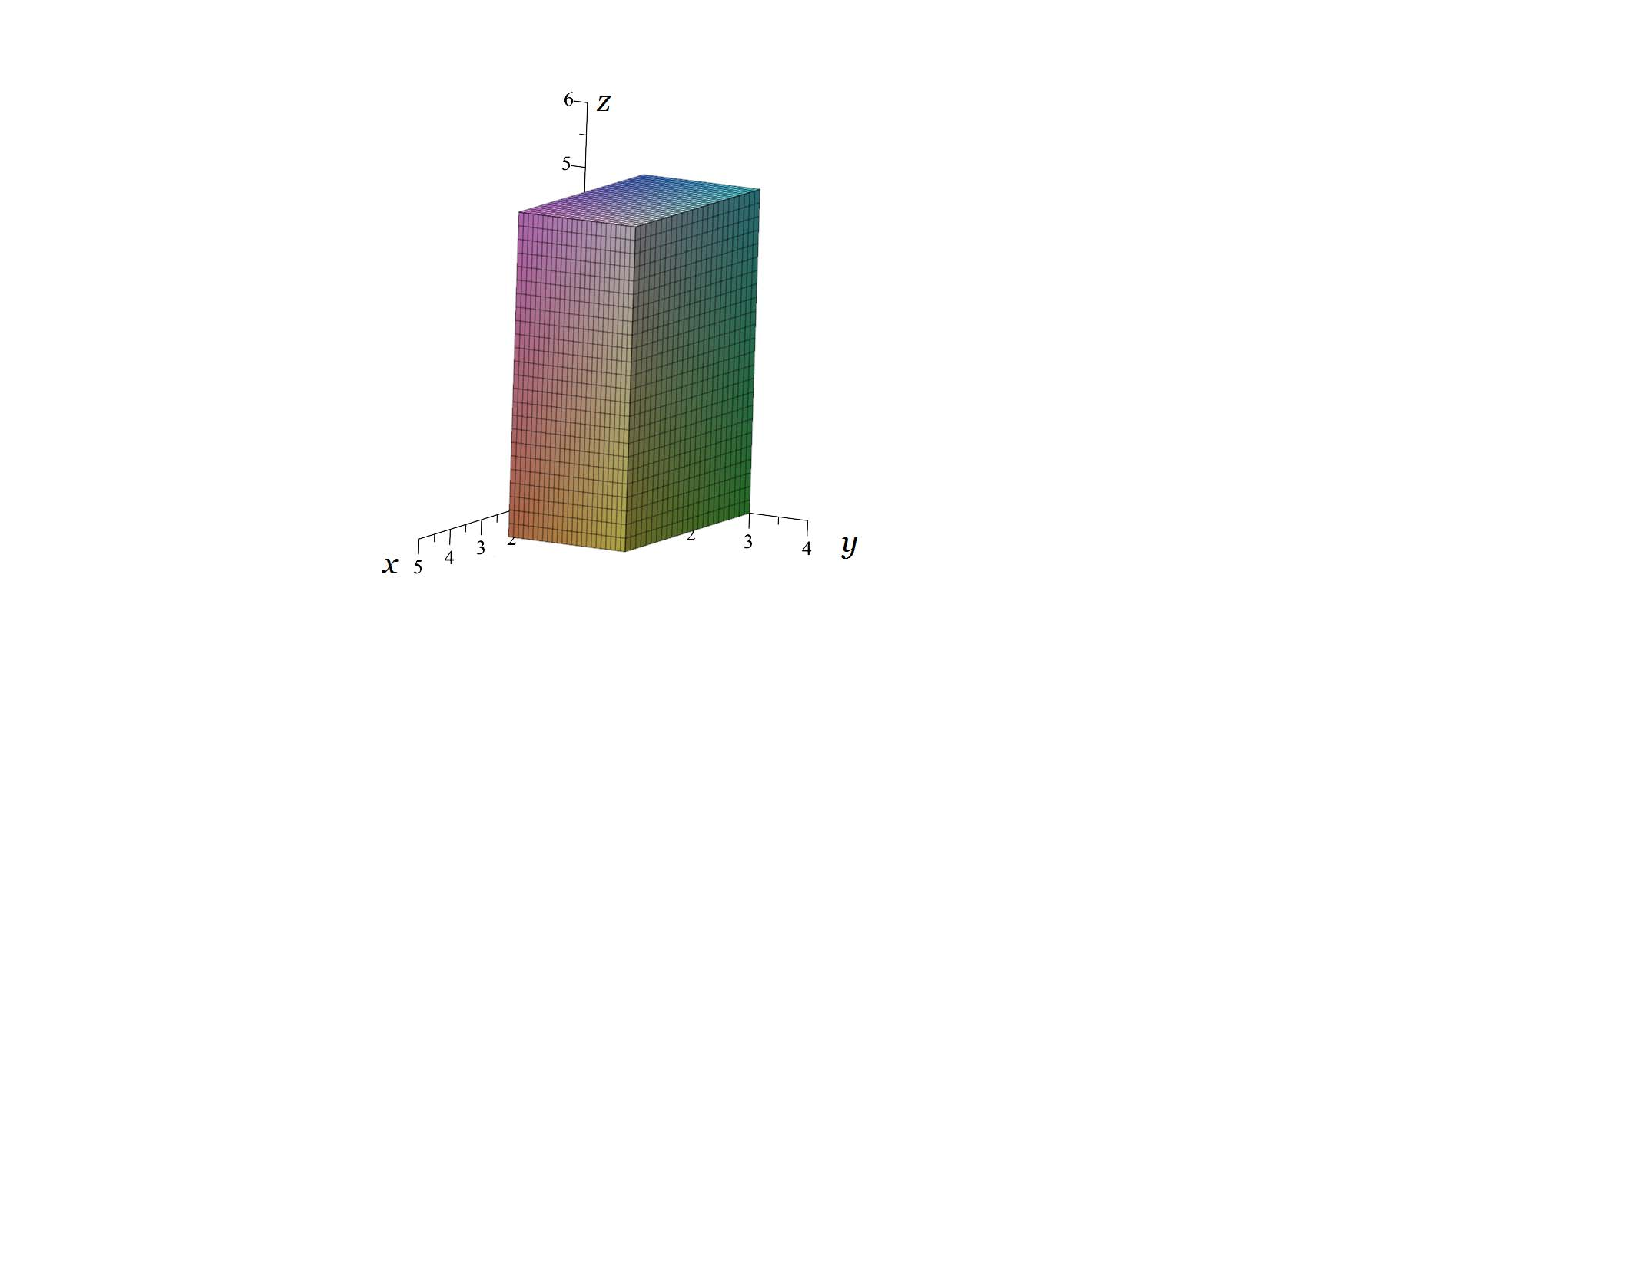
\includegraphics[scale=0.4]{box.pdf}
\end{center}
}}} \fi

\item $\int_0^2 \int_0^2 {(4-x-y)} \,dx \,dy$

\ifans{\fbox{\parbox{1\linewidth}{This value of this integral can be thought of as the volume between the plane $z=4-x-y$ and the $xy$-plane over the square $[0,2]\times[0,2]$.\\
\begin{center}
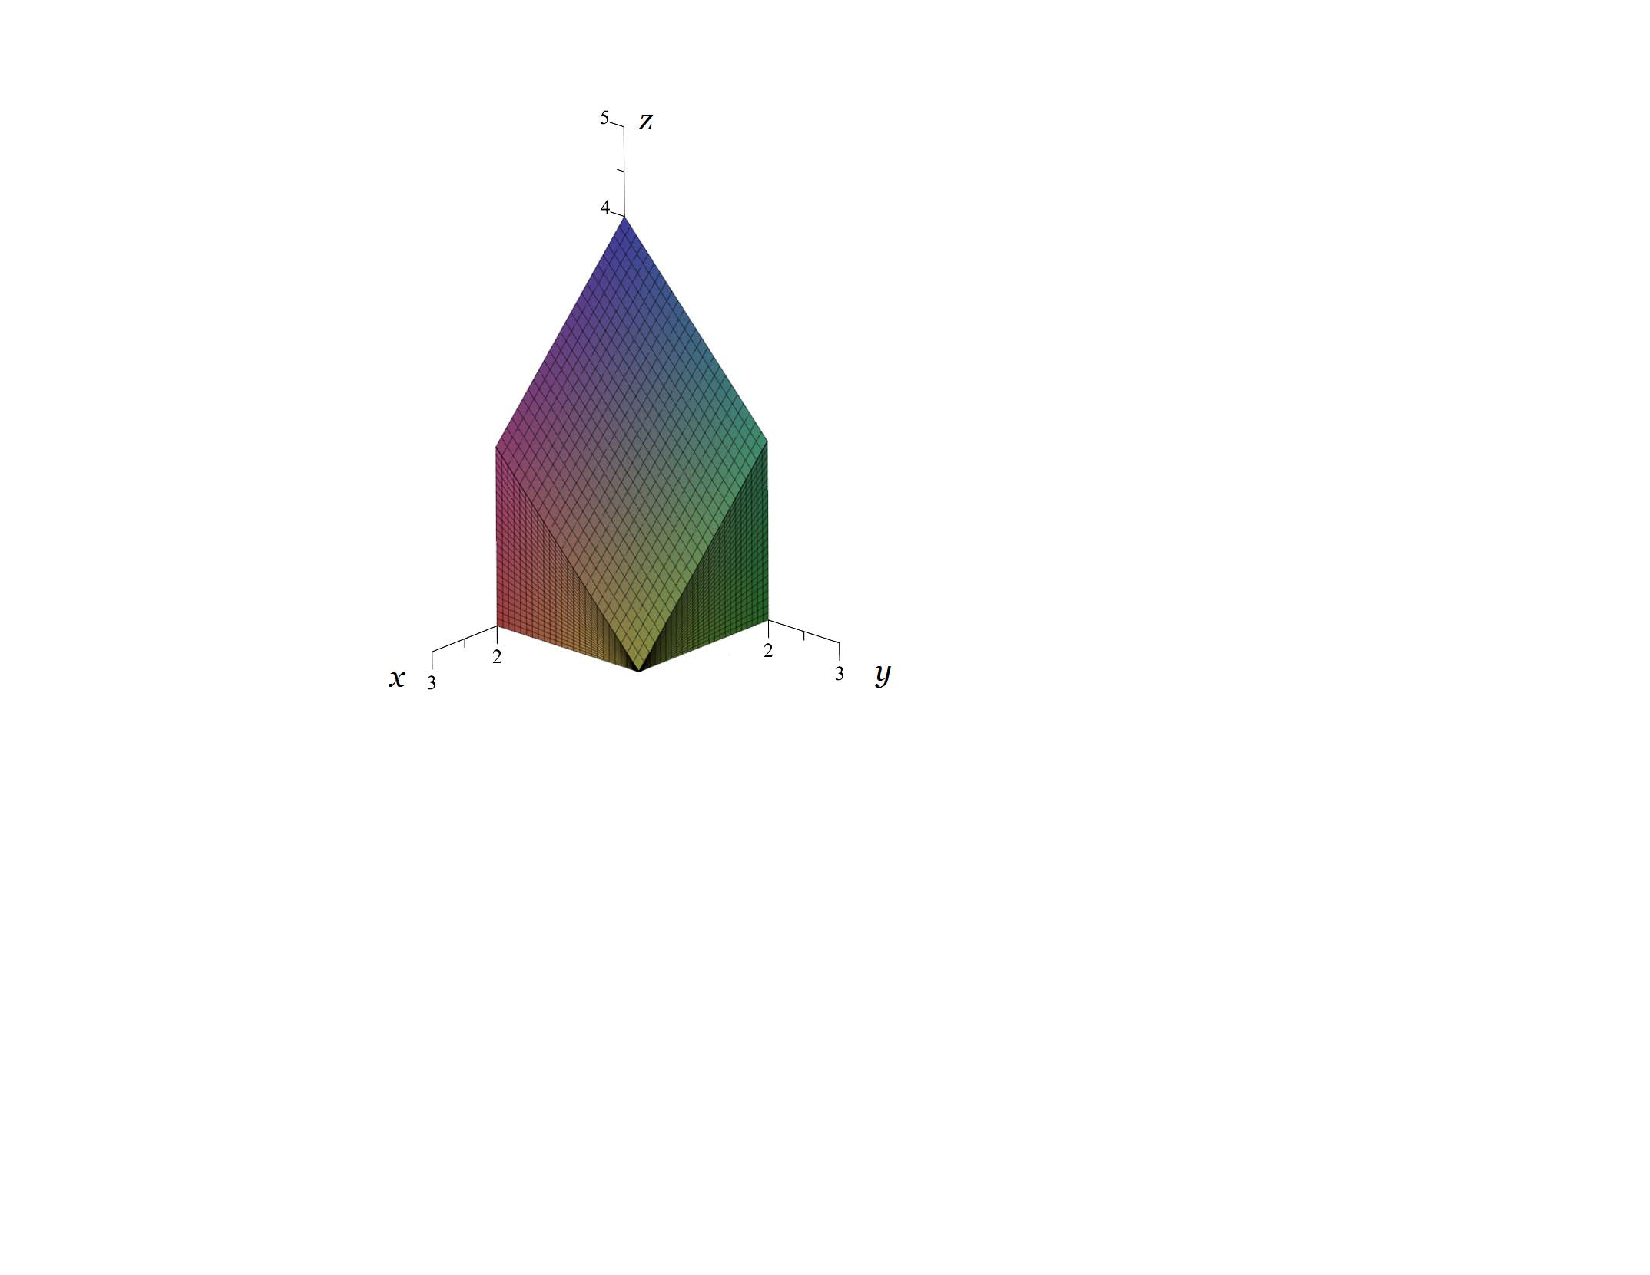
\includegraphics[scale=0.4]{plane.pdf}
\end{center}
}}} \fi

\end{enumerate}

\item Use a double integral to find the volume of the solid which is bounded by the circular paraboloid $z=x^2+y^2$ and the planes $z=0$, $x=0$, $x=4$, $y=0$, and $y=2$.

\ifans{\fbox{$\frac{160}{3}$}} \fi

\item Consider the rectangle $R$ in the $xy$-plane which has vertices $(0,1)$, $(0,4)$, $(3,1)$, and $(3,4)$.

\begin{enumerate}

\item Use a double integral to compute the area of $R$.

\ifans{\fbox{$A=\int_0^3\int_1^4 1 \,dy\,dx=\int_1^4\int_0^3 1 \,dx\,dy=9$}} \fi

\item Verify your answer from part (a) by using an appropriate formula from geometry.

\ifans{\fbox{$A=bh=3\cdot3=9$}} \fi

\end{enumerate}

\item By choosing a convenient order or integration, evaluate $\iint \limits_{R} x\sec^2{(xy)}\sec^2{x} \,dA$ where $R=\left\{(x,y) : \frac{\pi}{4}\leq x \leq \frac{\pi}{3}, 0 \leq y \leq 1\right\}$

\ifans{\fbox{1}} \fi

\end{enumerate}

\end{document}